% =============================================================
% fig_arch_fusion.tex
% Architecture diagram: Hybrid residual fusion (planned / future work)
% Compile standalone:  pdflatex fig_arch_fusion.tex
% =============================================================
\documentclass[tikz, border=8pt]{standalone}
\usepackage{amsmath,amssymb}
\usetikzlibrary{arrows.meta, positioning, fit, backgrounds, calc}

% ---- Shared colour palette (kept identical across all 4 architecture figures) ----
\definecolor{cInput}{HTML}{4477AA}    % blue    - input blocks
\definecolor{cSpatial}{HTML}{8855AA}  % violet  - spatial encoder
\definecolor{cGraph}{HTML}{EE9922}    % amber   - graph components
\definecolor{cTemporal}{HTML}{229988} % teal    - temporal encoder (LSTM)
\definecolor{cOutput}{HTML}{EE6677}   % coral   - output layer
\definecolor{cMuted}{HTML}{999999}    % grey    - "not used in this variant"

% ---- Shared node / arrow styles ----
\tikzset{
  font=\sffamily,
  block/.style={draw=black!70, rounded corners=3pt, line width=0.7pt,
    text width=2.0cm, align=center, font=\sffamily\footnotesize,
    minimum height=1.05cm, inner sep=3pt},
  inputblock/.style={block, fill=cInput!15, draw=cInput!75!black, text width=2.2cm},
  spatialblock/.style={block, fill=cSpatial!15, draw=cSpatial!75!black},
  graphblock/.style={block, fill=cGraph!22, draw=cGraph!80!black},
  neutralblock/.style={block, fill=black!4, draw=black!55},
  temporalblock/.style={block, fill=cTemporal!15, draw=cTemporal!75!black},
  headblock/.style={block, fill=black!4, draw=black!55, text width=2.4cm},
  outputblock/.style={circle, draw=cOutput!75!black, fill=cOutput!25,
    minimum size=1.1cm, font=\sffamily\small, line width=0.7pt},
  sumnode/.style={circle, draw=black!70, fill=black!8, minimum size=7mm,
    font=\sffamily\small, line width=0.8pt},
  flow/.style={-{Latex[length=2.4mm, width=1.8mm]}, line width=0.9pt, draw=black!70},
  dimlabel/.style={font=\scriptsize\itshape, text=black!60, align=center},
  grouplabel/.style={font=\bfseries\scriptsize, text=black!70, align=center},
  branchlabel/.style={font=\bfseries\scriptsize\itshape, align=center},
  groupbox/.style={draw=black!35, dash pattern=on 3pt off 2pt, rounded corners=4pt, inner sep=7pt},
  futurebox/.style={draw=black!50, dash pattern=on 5pt off 3pt, rounded corners=6pt,
    line width=1.1pt, inner sep=10mm},
}

\begin{document}
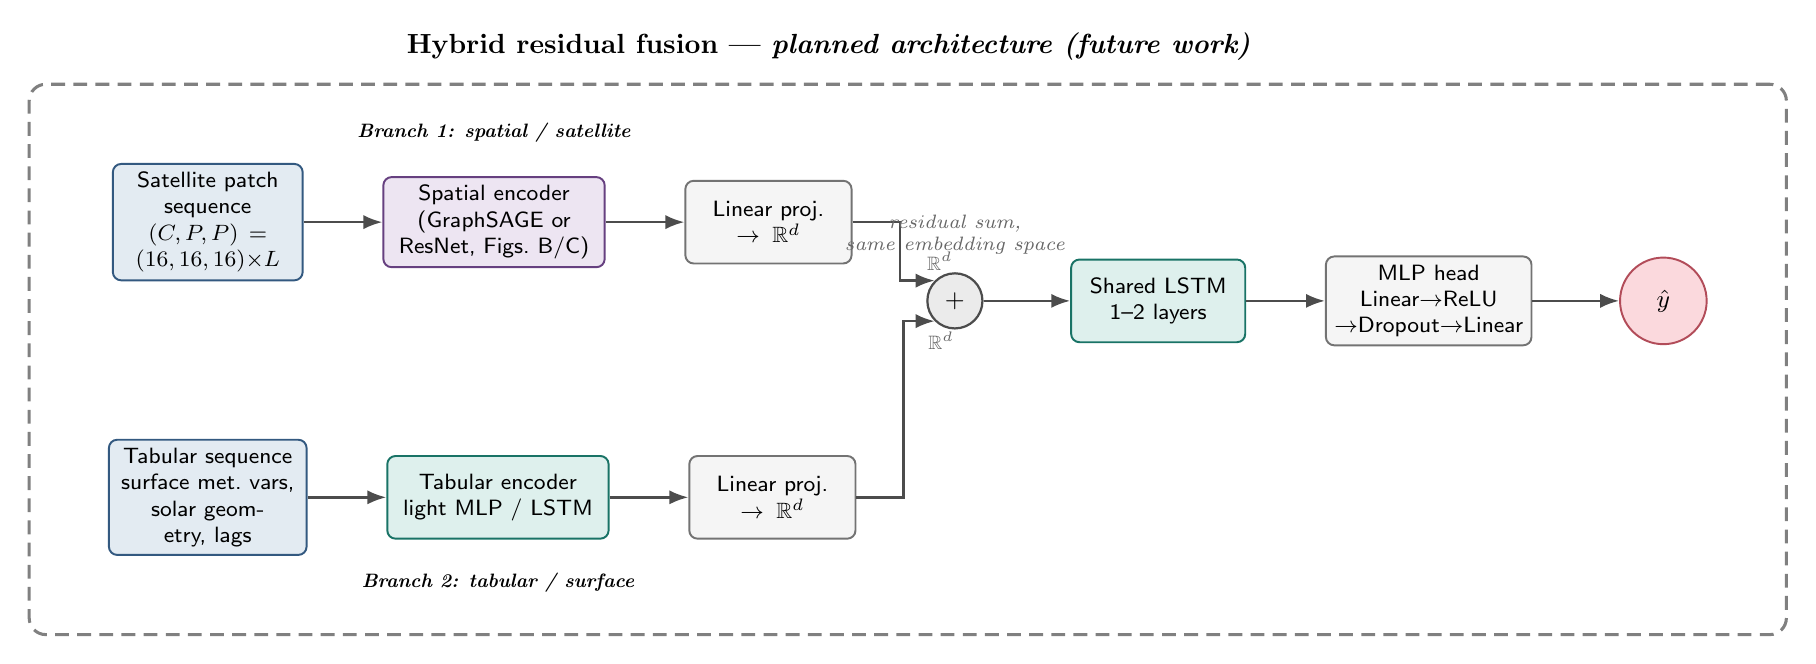
\begin{tikzpicture}[node distance=8mm]

  % ==================================================================
  % Branch 1 (top): spatial / satellite encoder  (GraphSAGE or ResNet)
  % ==================================================================
  \node[inputblock] (input1)
    {Satellite patch\\ sequence\\ \footnotesize $(C,P,P)=(16,16,16){\times}L$};

  \node[spatialblock, right=10mm of input1, text width=2.6cm] (spatialenc)
    {Spatial encoder\\ \footnotesize (GraphSAGE or ResNet, Figs.~B/C)};

  \node[neutralblock, right=10mm of spatialenc, text width=1.9cm] (proj1)
    {Linear proj.\\ $\to \mathbb{R}^{d}$};

  \node[branchlabel, above=3mm of spatialenc] {Branch 1: spatial / satellite};

  % ==================================================================
  % Branch 2 (bottom): tabular encoder (surface met + solar geometry + lags)
  % ==================================================================
  \node[inputblock, below=20mm of input1, text width=2.3cm] (input2)
    {Tabular sequence\\ \footnotesize surface met.\ vars,\\ solar geometry, lags};

  \node[temporalblock, right=10mm of input2, text width=2.6cm] (tabenc)
    {Tabular encoder\\ \footnotesize light MLP / LSTM};

  \node[neutralblock, right=10mm of tabenc, text width=1.9cm] (proj2)
    {Linear proj.\\ $\to \mathbb{R}^{d}$};

  \node[branchlabel, below=3mm of tabenc] {Branch 2: tabular / surface};

  % ==================================================================
  % Residual sum, shared LSTM, MLP head, output
  % ==================================================================
  \node[sumnode] (sum) at ($(proj1.east)+(13mm,-10mm)$) {$+$};

  \node[temporalblock, right=11mm of sum, text width=2.0cm] (lstm)
    {Shared LSTM\\ \footnotesize 1--2 layers};

  \node[headblock, right=10mm of lstm] (mlphead)
    {MLP head\\ \footnotesize Linear$\to$ReLU\\ $\to$Dropout$\to$Linear};

  \node[outputblock, right=11mm of mlphead] (out) {$\hat{y}$};

  % ----------------------------------------------------------------
  % Arrows
  % ----------------------------------------------------------------
  \draw[flow] (input1) -- (spatialenc);
  \draw[flow] (spatialenc) -- (proj1);
  \draw[flow] (input2) -- (tabenc);
  \draw[flow] (tabenc) -- (proj2);

  \draw[flow] (proj1.east) -| ($(proj1.east)+(6mm,0)$) |- (sum.north west)
    node[dimlabel, pos=0.85, above, xshift=2mm] {$\mathbb{R}^{d}$};
  \draw[flow] (proj2.east) -| ($(proj2.east)+(6mm,0)$) |- (sum.south west)
    node[dimlabel, pos=0.85, below, xshift=2mm] {$\mathbb{R}^{d}$};

  \draw[flow] (sum) -- (lstm);
  \draw[flow] (lstm) -- (mlphead);
  \draw[flow] (mlphead) -- (out);

  \node[dimlabel, above=1mm of sum] {residual sum,\\ same embedding space};

  % ----------------------------------------------------------------
  % Group box around the whole figure + "future work" badge
  % ----------------------------------------------------------------
  \node[futurebox, fit=(input1)(input2)(spatialenc)(tabenc)(proj1)(proj2)(sum)(lstm)(mlphead)(out)]
    (fbox) {};

  \node[font=\bfseries\normalsize, fill=white, inner sep=2pt,
        above=2mm of fbox.north, xshift=-10mm] (title)
    {Hybrid residual fusion --- \textit{planned architecture (future work)}};

\end{tikzpicture}
\end{document}
